\section{Prospection-Guided Retrieval}
\label{sec:method}

\begin{figure*}[t]
\centering
            \begin{minipage}[t]{0.9\textwidth}
            \vspace{-0.1in}
            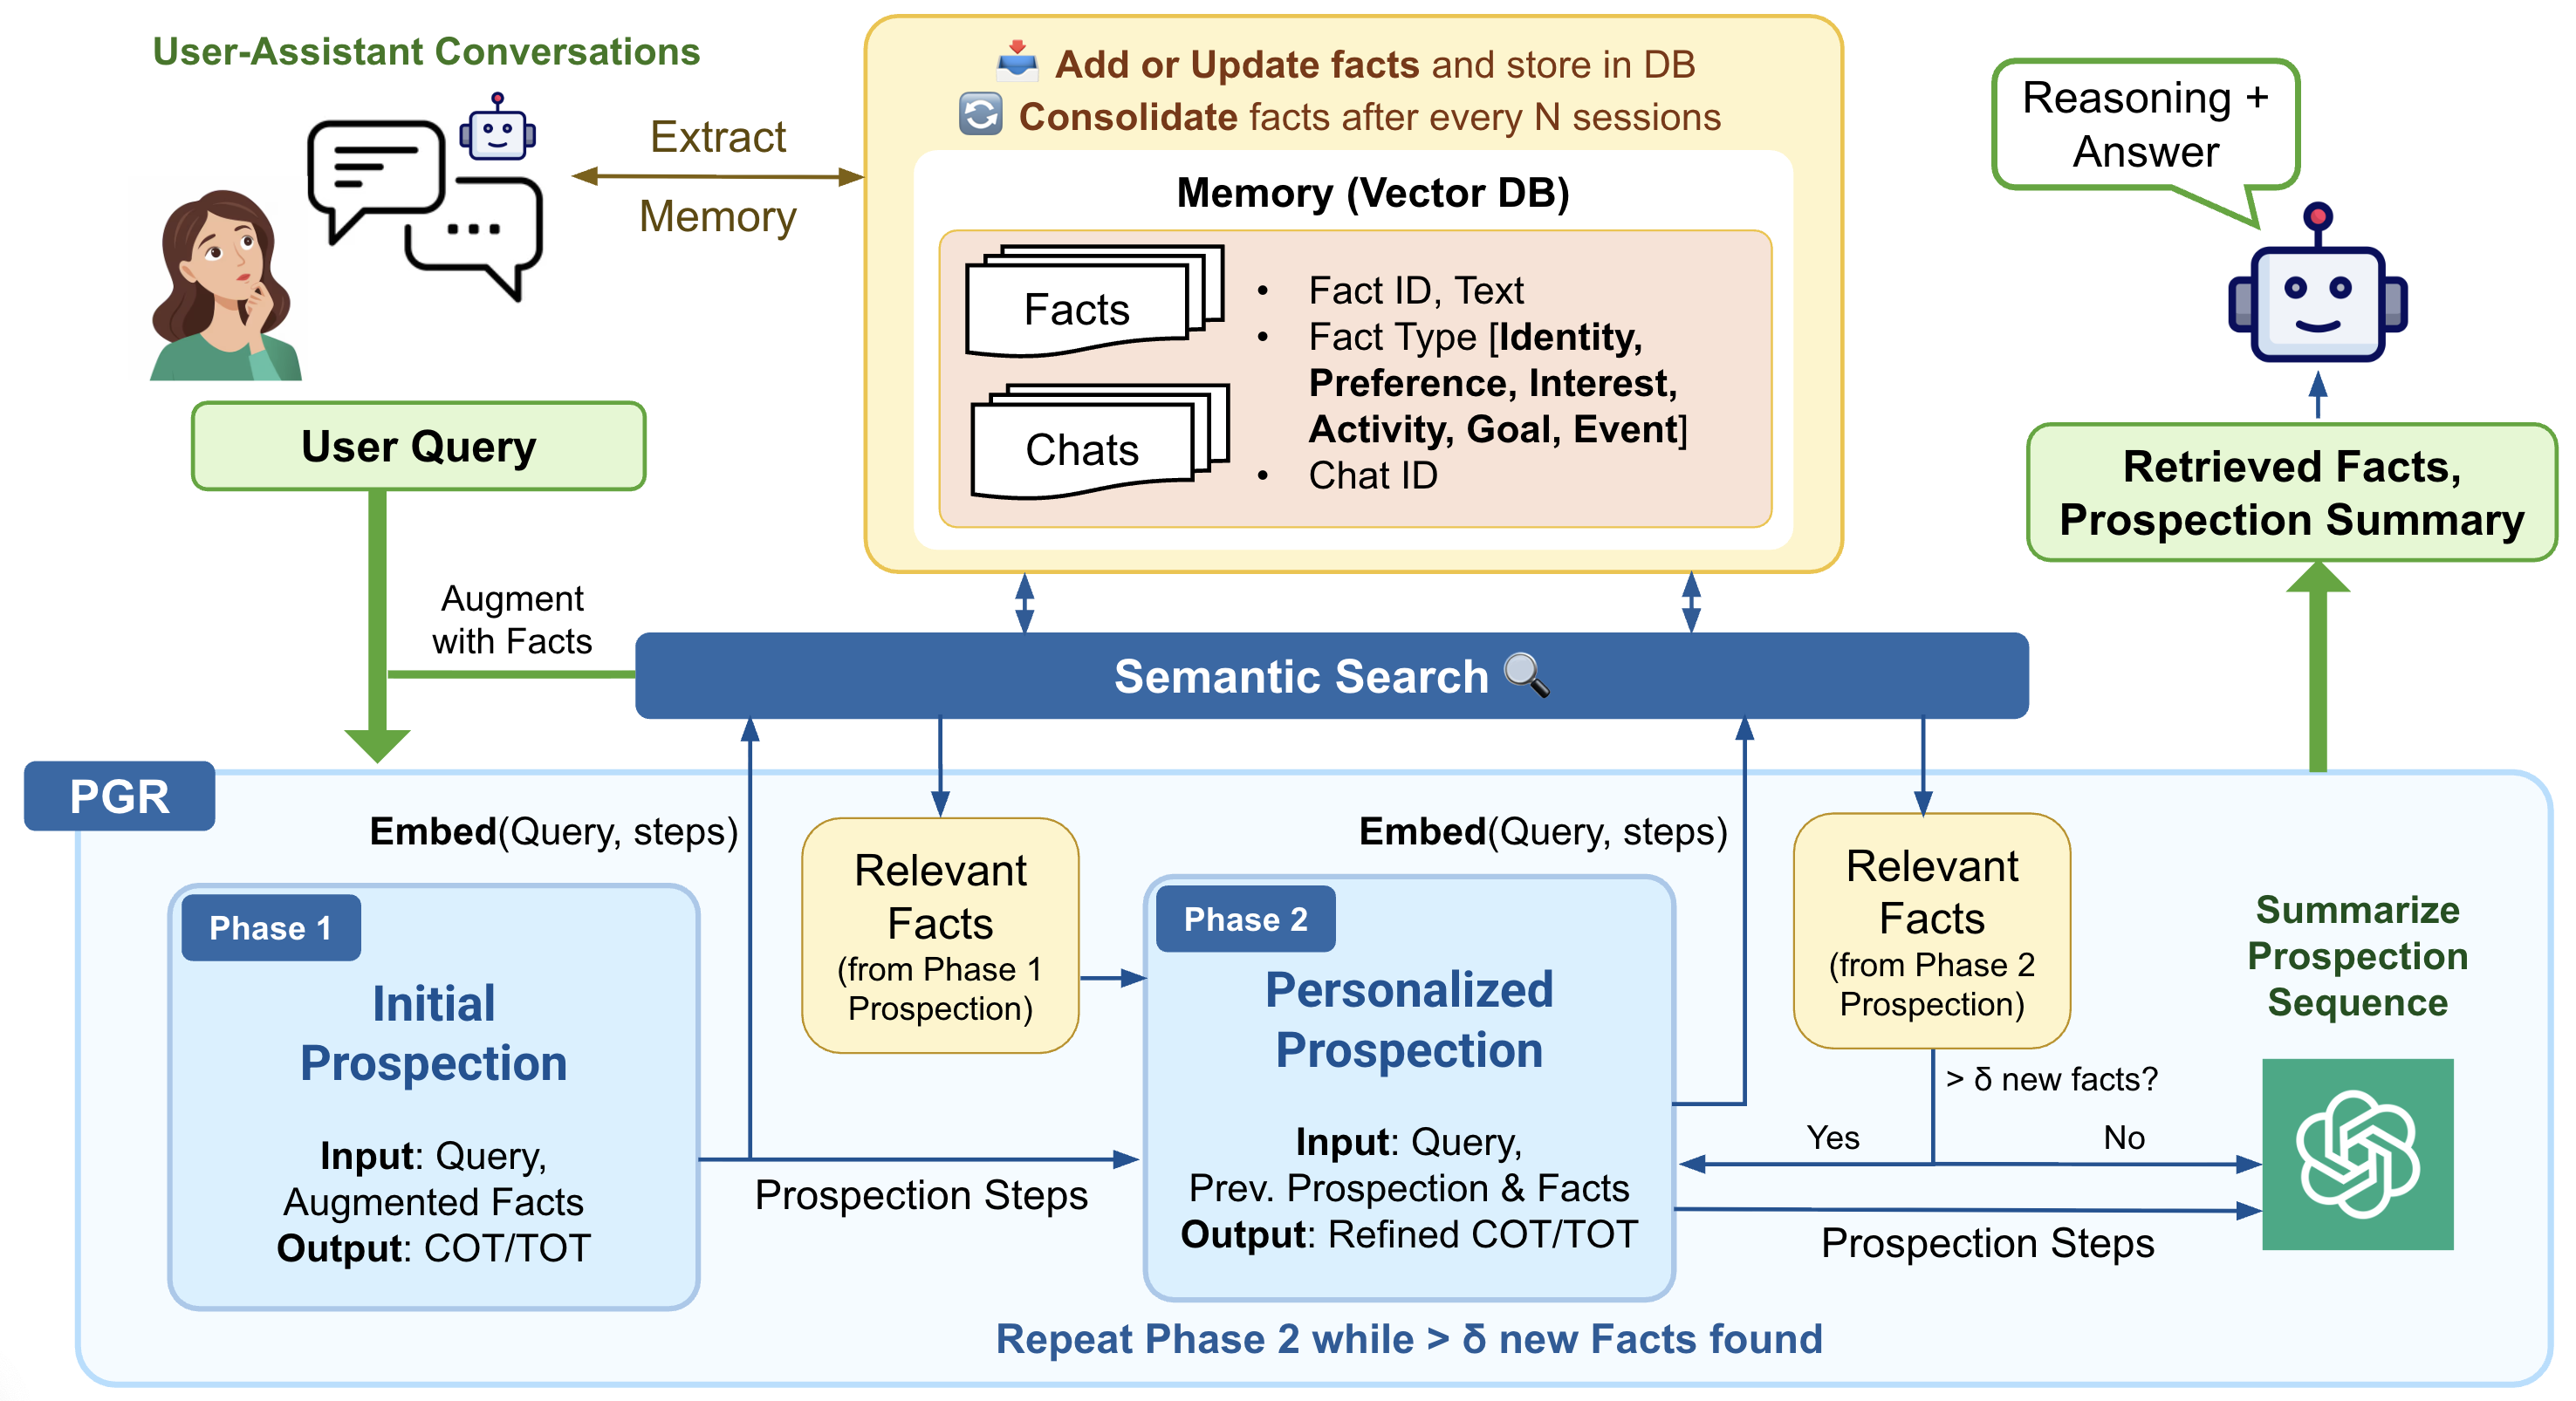
\includegraphics[width=\columnwidth]{figures/PGR-Overview.png}
            \vspace{-0.2in}
            \caption{\small{Overview of PGR}}
            \label{fig:pgr-fig}
            \end{minipage}
\end{figure*}

Inspired by the neurobiological dialogue between the prefrontal cortex and the hippocampus, Prospection-Guided Retrieval (PGR) operationalizes \emph{prospection}---the mental simulation of possible futures used to trigger the recall of contextually relevant memories~\cite{schacter2017episodic}. Unlike RAG and GraphRAG, which are anchored to a static ``lookup mentality'' dictated by storage structure, PGR treats memory as a substrate managed by an independent retrieval policy. Acting as an executive controller, PGR executes an iterative $\text{Simulate} \rightarrow \text{Retrieve} \rightarrow \text{Refine}$ loop to surface latent or counterfactual memories. This framework transforms archival records into a dynamic resource for real-time anticipatory intelligence.

\subsection{System Architecture Overview}
\label{sec:architecture}

As illustrated in Figure~\ref{fig:pgr-fig}, our architecture comprises three interconnected modules: the \textbf{Chat Interface}, \textbf{Long Term Memory}, and \textbf{PGR}.

\vspace{-0.2cm}
\paragraph{Chat Interface.} 
The assistant interacts with the user via a standard dialogue interface. Queries are sent to PGR, which returns relevant facts and a prospection reasoning summary. This summary enables the agent to generate responses that are both factually grounded and anticipatory.

\vspace{-0.2cm}
\paragraph{Long Term Memory.} 
Analogous to the hippocampus, this layer maintains long-term knowledge across sessions. Our reference implementation uses a structured fact-store with periodic consolidation, but the system is substrate-agnostic. PGR accesses it via a standard query interface (e.g., vector or graph similarity) as a black-box resource for simulations.

Serving as a computational prefrontal cortex, PGR mediates between interface and memory. It executes an iterative retrieval process, generating future trajectories and grounding them in memory to identify contextually vital information. The module returns both retrieved memories and the prospection reasoning that guided their selection, enabling the agent to produce anticipatory responses.

\subsection{Long Term Memory}
\label{sec:pgr-memory}
The memory store maintains the agent's knowledge of the user across sessions. PGR is agnostic to the underlying storage technology and requires only a queryable memory interface; the backend may be a vector index, a knowledge graph, or a hybrid store. Our implementation uses two structures: \emph{conversation logs} and \emph{memory facts}.

\vspace{-0.2cm}
\paragraph{Conversation logs.} Each user--agent session is stored as a multi-turn conversation with a unique id and date. These logs merely serve as the source for memory fact extraction but not used for retrieval.

\vspace{-0.2cm}
\paragraph{Memory facts.} Facts are short, atomic statements extracted from conversations \eg demographics, preferences, plans, past events. Each fact is associated with a unique id, a type, a frequency count, related entities, and provenance (the sessions from which it was derived). Six types are used: Identity (demographics, profession, education, relationships); Preference (likes and habits); Goal (plans and upcoming events); Interest (hobbies and topics); Activity (recurring or past actions); and Event (situations or milestones that affect decisions). Extraction and each write are performed by an LLM; memory is updated once every few sessions to limit cost.

\vspace{-0.2cm}
\paragraph{Memory Upsert} For the first conversation, all extracted facts are treated as new and receive new identifiers. For subsequent conversations, extracted facts are upserted \ie only new facts are inserted while pre-existing ones are updated if necessary. 

\vspace{-0.2cm}
\paragraph{Memory Consolidation.} When the new fact count reaches a threshold (50 new facts since the last merge), facts are merged based on semantic similarity and temporal proximity. Fact texts are embedded and clustered by cosine similarity; within each cluster, only facts whose most recent date falls within a fixed time window (7 days) are merged. An LLM consolidates each such group into a single fact; provenance is aggregated and the original identifiers are retained.

\vspace{-0.2cm}
\paragraph{Retrieval.} At query time, retrieval is performed over the memory facts by embedding-based similarity (like a RAG); PGR applies its prospective loop on top of this interface. 

\noindent
All the prompts used for extraction, update, and merge are provided in Appendix~\ref{sec:appendix}.


\subsection{Prospection Guided Retrieval}
\label{sec:pgr-retrieval}

The core of PGR is an iterative \emph{simulate--retrieve--refine} process that mirrors human prospection. Rather than treating a user query as a static search term, PGR treats it as a starting point for mental simulation. The underlying intuition is that to find a memory that is logically relevant but semantically distant, the system must first ``imagine'' the future scenarios where that memory would be required. 

This mechanism acts as a dynamic dialogue between a generative planner (the PFC analog) and the memory substrate (the hippocampal analog). The process begins with a query augmentation step to ground the user intent, followed by two phases of prospection that iteratively retrieve and refine relevant memories:

\squishlist
    \item \textbf{Initial Prospection (Phase 1):} The system generates a broad ``horizon'' of potential future actions. This simulation can be operationalized as either a linear \textit{Chain-of-Thought (CoT)} or a branching \textit{Tree-of-Thought (ToT)} structure. Each hypothesized step serves as an independent \textbf{sub-query} to the memory store, potentially surfacing latent facts that the original query alone would fail to trigger. 
    \item \textbf{Personalized Prospection (Phase 2):} The system refines the simulation by conditioning it on the facts retrieved in Phase 1. This personalization allows the simulation to reflect user-specific constraints, proactively retrieving memories that match the refined context.
\squishend

This iterative loop ensures that each retrieved memory informs a more accurate simulation of the future, which in turn serves as a more precise probe for deeper, latent memories. 

\paragraph{Formal Setup.}
Let $\mathcal{M}$ denote the memory store. 
% To ensure temporal validity, we restrict $\mathcal{M}$ to facts whose timestamp $t \leq t_{\text{query}}$. 
The memory substrate is defined via an abstract retrieval function $\phi(x; \mathcal{M}, \Theta)$, returning a set of facts relevant to a sub-query $x$. In our reference implementation, $\Theta = \{K, \tau\}$, representing the top-$K$ facts above semantic similarity threshold $\tau$. For different memory architectures, $\Theta$ may instead encode traversal depth, temporal windows, or community hierarchy. We denote $R$ as the set of accumulated facts, initially $R = \emptyset$.

\paragraph{Query Augmentation.} 
PGR first generates an augmented query $q_A$ to resolve underspecified user queries by retrieving tightly relevant context:
\vspace{-.8em}
\begin{equation}
q_A = \mathrm{LLM}(P_A(q,\, \phi(q;\mathcal{M}, \Theta_o)))
\end{equation}

where $P_A$ instructs the model to disambiguate using context $\Theta_o$ (e.g., $K_o, \tau_o$). This ensures the simulation begins with a high-fidelity representation of user intent.

\paragraph{Phase 1: Initial Prospection.} 
The LLM processes $q_A$ to produce a prospection sequence $S^0 = \{s^0_1, \ldots, s^0_L\}$ of hypothesized subgoals or future contexts:
\vspace{-.8em}
\begin{equation}
S^0 = \mathrm{LLM}(P_{\mathrm{sim}}(q_A))
\end{equation}

Each $s^0_l \in S^0$ is used as a sub-query to the memory store, and retrieved facts are merged with the initial query results:
\vspace{-.8em}
\begin{equation}
R \leftarrow \phi(q;\mathcal{M}, \Theta) \cup \bigcup_{l=1}^{L} \phi(s^0_l;\mathcal{M}, \Theta)
\end{equation}

\paragraph{Phase 2: Personalized Prospection.} 
Using the accumulated knowledge $R$, the LLM iteratively refines the prospection sequence, making it personalized to the user:
\begin{equation}
S^i = \mathrm{LLM}(P_{\mathrm{ref}}(q_A, R, S^{i-1}))
\end{equation}

For each refined sub-query $s^i_l \in S^i$, similar facts are retrieved. $\Delta^i$ denotes the set of unique, previously unseen facts discovered during iteration $i$:
\vspace{-.8em}
\begin{equation}
\Delta^i = \bigcup_l \phi(s^i_l;\mathcal{M}, \Theta) \setminus R
\end{equation}

The memory set is updated $R \leftarrow R \cup \Delta^i$, and the loop terminates when $|\Delta^i|$ falls below a convergence threshold $\delta$ or a maximum iteration $I_{\max}$ is reached. The final set $R^*$ is returned alongside a prospection reasoning summary detailing how the simulation guided memory recall.



\begin{algorithm}[t]
\caption{Prospection-Guided Retrieval (PGR)}
\label{alg:pgr}
\begin{algorithmic}[1]
\Require Query $q$, memory store $\mathcal{M}$, abstract retrieval function $\phi$, augmentation parameters $\Theta_o$, retrieval parameters $\Theta$, convergence threshold $\delta$, max iterations $I_{\max}$
\Ensure Final retrieved fact set $R^*$

\State $R \leftarrow \emptyset$
\State \Comment{\textit{Query Augmentation}}
\State $q_A \leftarrow \mathrm{LLM}(P_A(q,\; \phi(q;\mathcal{M}, \Theta_o)))$

\State \Comment{\textit{Phase 1: Initial Prospection}}
\State $S^0 \leftarrow \mathrm{LLM}(P_{\mathrm{sim}}(q_A))$
\State $R \leftarrow \phi(q;\mathcal{M}, \Theta) \;\cup \displaystyle\bigcup_{l=1}^{|S^0|} \phi(s^0_l;\mathcal{M}, \Theta)$

\State \Comment{\textit{Phase 2: Personalized Prospection}}
\For{$i = 1, 2, \ldots, I_{\max}$}
    \State $S^i \leftarrow \mathrm{LLM}(P_{\mathrm{ref}}(q_A,\, R,\, S^{i-1}))$
    \State $\Delta^i \leftarrow \displaystyle\bigcup_{l=1}^{|S^i|} \phi(s^i_l;\mathcal{M}, \Theta) \;\setminus\; R$
    \State $R \leftarrow R \cup \Delta^i$
    \If{$|\Delta^i| < \delta$} \textbf{break} \EndIf
\EndFor
\State \Return $R^* \leftarrow R$
\end{algorithmic}
\end{algorithm}
